\documentclass[a4paper]{article}
\usepackage{parskip} % For paragraph layout
\usepackage{setspace} % For using single or double spacing
\usepackage{emptypage} % To insert empty pages
\setlength\parindent{0pt} % Indentation
\raggedbottom  
% PACKAGES FOR TITLES
\usepackage{titlesec}
% \titlespacing{\section}{left spacing}{before spacing}{after spacing}
\titlespacing{\section}{0pt}{3.3ex}{2ex}
\titlespacing{\subsection}{0pt}{3.3ex}{1.65ex}
\titlespacing{\subsubsection}{0pt}{3.3ex}{1ex}
\usepackage[utf8]{inputenc}
\usepackage[italian]{babel}
\usepackage[T1]{fontenc} % Font encoding
\usepackage[11pt]{moresize} % Big fonts
\usepackage{csquotes}
\usepackage{graphicx}
\usepackage{float}
\usepackage{listings}
\usepackage{xcolor}
\usepackage{algorithm}
\usepackage{algorithmic}
\usepackage{afterpage}
\usepackage{lipsum} % DUMMY PACKAGE
\usepackage{fancyhdr} % For the headers
\usepackage[backend=biber]{biblatex}
\addbibresource{bibliography.bib}
\nocite{*}
\addto\captionsitalian{%
  \renewcommand{\lstlistingname}{Listato}%
  \renewcommand\lstlistlistingname{Listati}}

\definecolor{codegreen}{rgb}{0,0.6,0}
\definecolor{codegray}{rgb}{0.5,0.5,0.5}
\definecolor{codepurple}{rgb}{0.58,0,0.82}
\definecolor{backcolour}{rgb}{0.95,0.95,0.92}
\lstdefinestyle{mystyle}{
    backgroundcolor=\color{backcolour},   
    commentstyle=\color{codegreen},
    keywordstyle=\color{magenta},
    numberstyle=\tiny\color{codegray},
    stringstyle=\color{codepurple},
    basicstyle=\ttfamily\footnotesize,
    breakatwhitespace=false,         
    breaklines=true,                 
    captionpos=b,                    
    keepspaces=true,                 
    numbers=left,                    
    numbersep=5pt,                  
    showspaces=false,                
    showstringspaces=false,
    showtabs=false,                  
    tabsize=2
}

\lstset{style=mystyle}
\begin{document}



\clearpage
\null
\thispagestyle{empty}
\clearpage

\section*{Abstract}
Una sfida fondamentale per gli standard che trattano dati sanitari è la gestione della grande variabilità causata dai molteplici tipi di processi e prodotti. \\
Spesso, molti campi e opzioni possono essere aggiunti alla specifica, risultando così in un aumento graduale di costi e complessità del sistema da realizzare. \\
Un'alternativa potrebbe essere la creazione di estensioni dedicate, ma anche questa comporta molti problemi di implementazione.
\\
La maggior parte dei database sanitari utilizzano il protocollo FHIR, diffuso in tutto il mondo e su cui è basato anche il fascicolo sanitario di Regione Lombardia. 
\\
Questo progetto di tesi ha avuto come oggetto di studio la prima parte del flusso di informazioni, relativa alla gestione da parte di dispositivi gateway (cellulari, personal computer) dei dati sanitari provenienti da dispositivi medici.\\
Si è dunque realizzato un progetto Java per la simulazione della creazione di dati seguendo lo standard IEEE 11073-10206 ACOM da parte di dispositivi medici e la successiva conversione nello standard FHIR.


\clearpage
\null
\thispagestyle{empty}

\clearpage

\tableofcontents
\newpage
\section{Introduzione}
\subsection{Scopo}
Oggetti come smartwatch, fasce cardio, bilance e termometri cosiddetti "intelligenti" stanno prendendo sempre più piede nelle vite della gente comune.
Come altri prodotti di consumo però esistono ovviamente diversi produttori sul mercato ed ognuno sviluppa il proprio protocollo ed applicativo dedicati
per gestire la comunicazione e la visualizzazione dei dati sanitari.
Questa tendenza rischia di non sfruttare le potenzialità in ambito sanitario che questi rilevatori di parametri vitali offrono, poiché potrebbero essere
utili in futuro grazie allo sviluppo della \textbf{telemedicina}.
Facciamo un esempio: una persona con una malattia cronica, come ad esempio il diabete, utilizza un rilevatore smart per tenere la glicemia sotto controllo.
I dati prodotti sono visualizzabili nell'applicazione del prodotto, risultando così "confinati".
Attraverso un sistema unico invece, si potrebbe utilizzare il dispositivo che riceve ed elabora i dati (cellulare personale, pc) come gateway, cioè come intermediario tra tutti i dispositivi
medici indossabili e un sistema remoto di storage ed elaborazione di dati sanitari, come il fascicolo sanitario.
In questo modo, la grande quantità di dati potrebbe essere analizzata in caso di bisogno dal personale medico, contribuendo a tracciare un quadro completo dello stato di salute dei pazienti.
\subsection{Obiettivi}
Sviluppo di un progetto Java che simula la creazione di dati da parte di dispositivi medici (osservazioni) seguendo le direttive dello standard IEEE 11073-10206 - ACOM e li converte nello
standard FHIR allo scopo di favorire l'interoperabilità tra sistemi differenti.
Sviluppo di un convertitore da ACOM a FHIR, prendendo in esame alcuni dispositivi specifici e le osservazioni che possono generare. 
\section{Background}
\subsection{IEEE 11073-10206 - ACOM}
\subsubsection{Ambito e finalità}
Questo standard definisce un modello di contenuto astratto (ACOM: Abstract Content Information Model) per i dispositivi di salute personale.
L'obiettivo di IEEE 11073-10206 è quello di documentare le informazioni in un Personal Health Device, da qui in poi chiamato PHD e il contenuto delle osservazioni sanitarie che vengono inviati dal PHD in modo che quando un'osservazione viene ricevuta dal PHD, indipendentemente dal protocollo utilizzato per eseguire
la comunicazione, le informazioni sanitarie sono \textbf{complete}, \textbf{coerenti} e \textbf{inequivocabili}.
IEEE 11073-10206 definisce un modello informativo astratto ed object-oriented allo scopo di rappresentare un PHD e le osservazioni che può generare.
Specifica quali informazioni devono essere presenti e le relazioni tra elementi informativi nel modello. Modella le osservazioni in modo generico
concentrandosi sulle informazioni contenuto nella presentazione delle misure sanitarie.
La figura~\ref{fig:overallContextOfWork} mostra le categorie e i tipi tipici di dispositivi nell'ambito della salute personale. I PHD (ad esempio: monitor della pressione sanguigna, bilance e pedometri) raccolgono informazioni su una o più persone, trasferendole poi ad un PHG, Personal Health Gateway (ad esempio: telefono cellulare, apparecchio sanitario o pc) per la raccolta, la visualizzazione e l'eventuale trasmissione successiva. Il PHG può anche trasmettere i dati a servizi di supporto remoto per ulteriori analisi o per permettere la gestione delle malattie.

\begin{figure}[H]
    \centering
    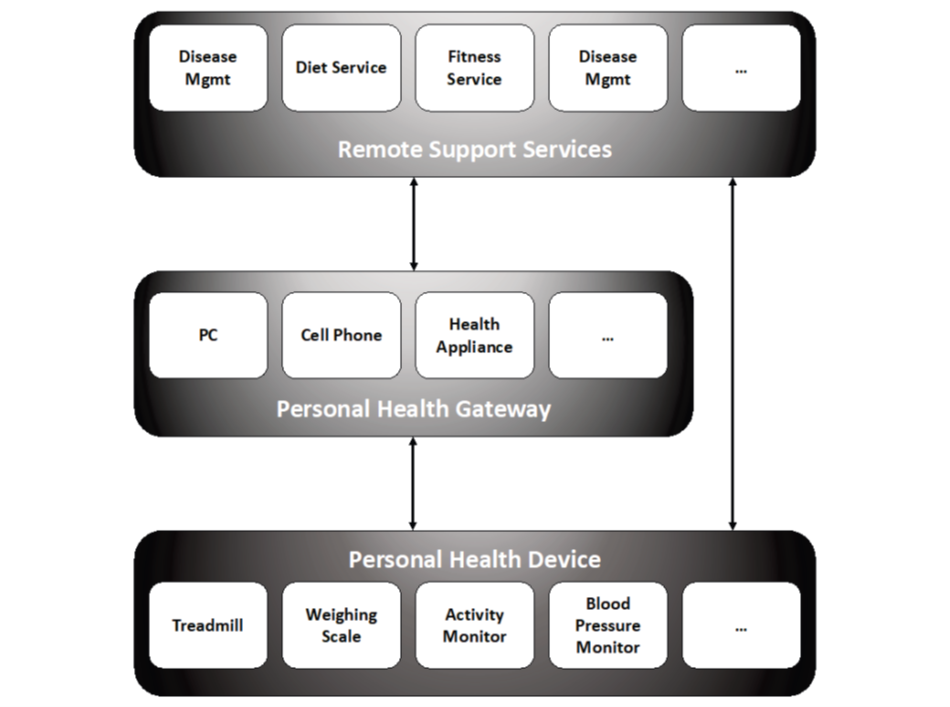
\includegraphics[width=1\textwidth]{figures/overall context of work.png}
    \caption{Contesto di ACOM}
    \label{fig:overallContextOfWork}
\end{figure}

\subsubsection{Classe Osservazione}
La classe di osservazione ACOM fornisce un modello generico per esprimere osservazioni da dispositivi di salute personale.
\'E basata sull'oggetto metrico descritto dallo standard ISO/IEEE 11073-20601 e condivide molti attributi della risorsa analoga osservazione presente nello standard HL7 FHIR.
Come si può vedere in figura \ref{fig:observationClass}, la classe si compone di una serie di elementi concettuali, tutti derivanti dall'oggetto \textbf{Observation}.

\begin{figure}[H]
    \centering
    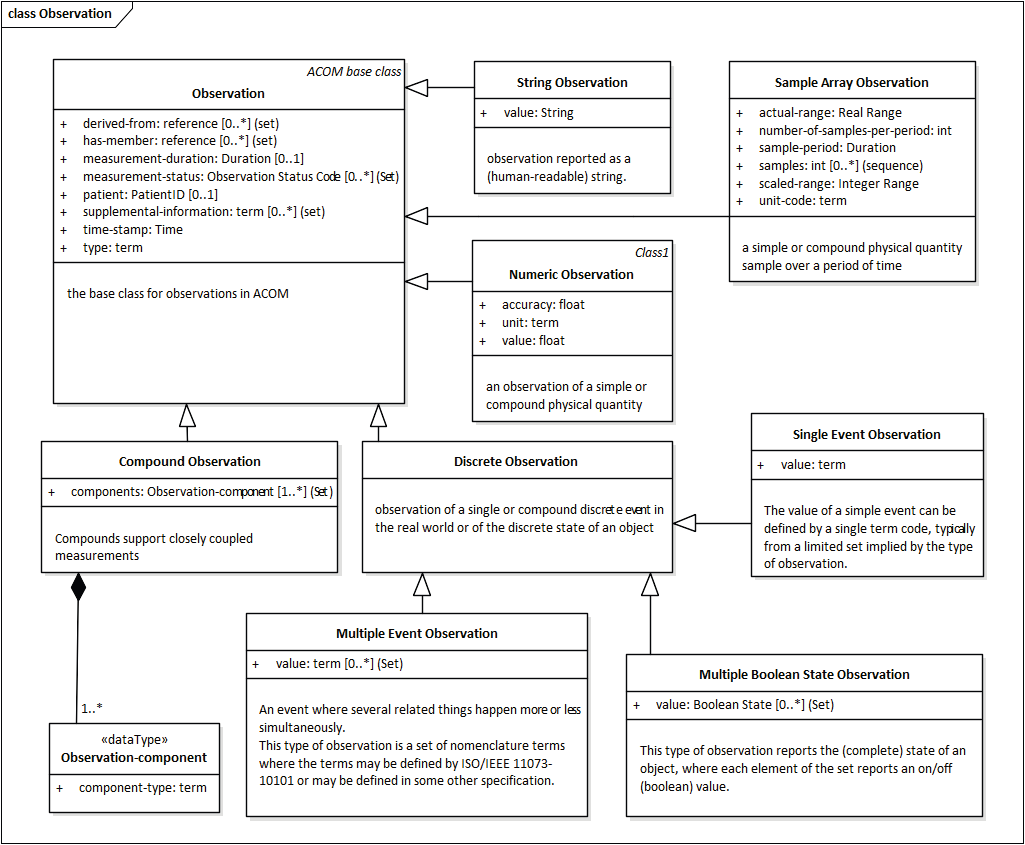
\includegraphics[width=1\textwidth]{figures/observation class.png}
    \caption{Classe Observation}
    \label{fig:observationClass}
\end{figure}

\subsubsection{Specializzazioni su dispositivi}
Le specializzazioni dei dispositivi sono usate in questo standard per definire il contenuto informativo di uno specifico tipo di PHD. 
Sono classi che modellano alcuni tipi di PHD particolari (appartenenti alla classe IEEE 11073-104XX), di conseguenza contengono al loro interno le informazioni basilari sulla struttura del PHD: \textbf{Power} rappresenta il tipo di alimentazione e le operazioni che mantengono in attività il PHD; \textbf{Clock} il riferimento di tempo che viene utilizzato per creare le osservazioni e \textbf{SystemInfo}, che rappresenta tutte le informazioni del sistema da emulare.
Vengono ora presentate due specializzazioni: IEEE 11073-10408 Termometro e IEEE 11073-10415 Bilancia con altimetro. è possibile notare grazie ai due diagrammi UML come i due dispositivi producano osservazioni differenti in tipo e quantità.

\begin{figure}[H]
    \centering
    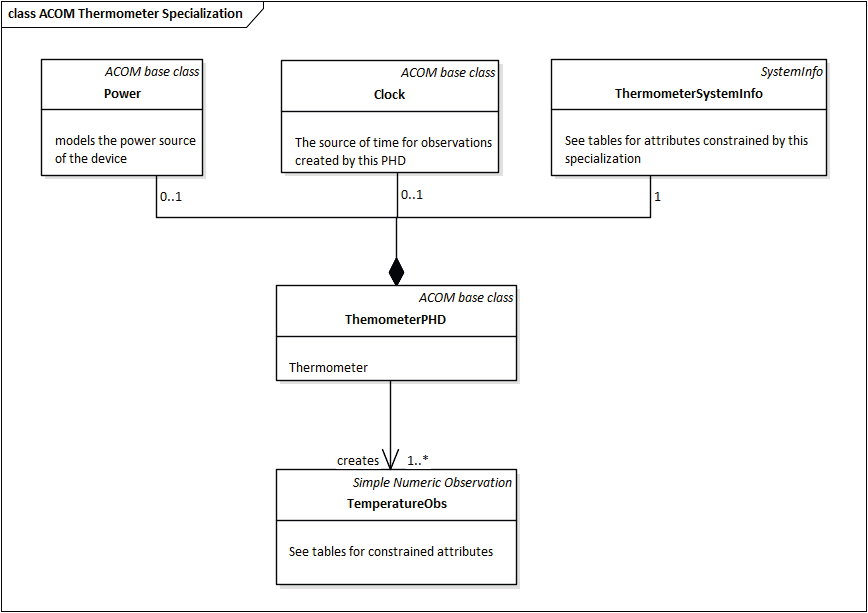
\includegraphics[width=1\textwidth]{figures/ACOM thermometer specialization class.png}
    \caption{classe ACOM che modella il dispositivo Termometro}
\end{figure}
\begin{figure}[H]
    \centering
    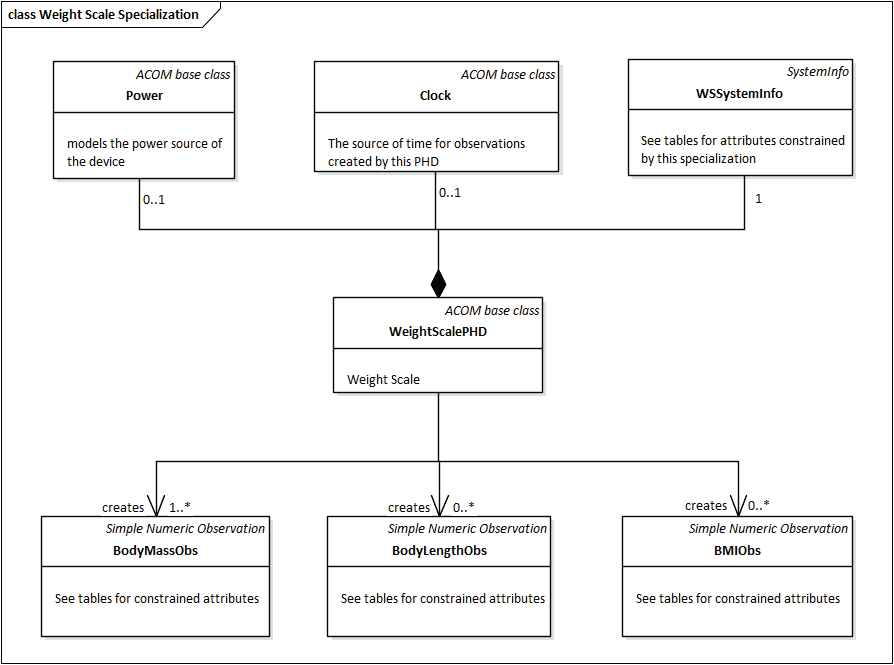
\includegraphics[width=1\linewidth]{figures/weightscale.png}
    \caption{classe ACOM che modella il dispositivo Bilancia con altimetro}
    \label{fig:enter-label}
\end{figure}
\subsection{FHIR}\label{subsec: FHIR}
\textbf{FHIR}, Fast Healthcare Interoperability Resources, è uno standard di interoperabilità sanitaria di HL7 (associazione non profit internazionale che si occupa di gestire standard per la sanità)
che consente a una moltitudine di sistemi di scambiare informazioni sanitarie utilizzando modelli di dati concordati. In FHIR, questi modelli di dati sono semplici, diretti, contemporaneamente
leggibili da uomo e computer e, quando combinati, abbastanza robusti da trasmettere informazioni sanitarie complesse.
Gli obbiettivi primari di FHIR sono:
\begin{itemize}
    \item creare uno standard da utilizzare tra diverse piattaforme informatiche che si occupano di dati sanitari
    \item rendere l'interoperabilità in tempo reale più semplice
\end{itemize}
In definitiva, FHIR riduce la curva d'apprendimento, rende l'interoperabilità più semplice e permette di creare in modo più veloce e semplice applicativi.

\subsubsection{Struttura}
Il componente base dello standard FHIR è la struttura chiamata \textbf{risorsa}. Tutti gli oggetti FHIR che possono essere inviati sono definiti come risorsa.
La filosofia su cui si basa FHIR è costruire un set base di risorse che, sia da sole sia combinate, possano soddisfare la maggioranza dei casi d'uso esistenti.
La modellazione FHIR usa un approccio compositivo, cioè implementa i casi d'uso combinando insieme più risorse singole.

\subsubsection*{Risorse}
In FHIR, i dati sanitari sono divisi in categorie, come ad esempio pazienti, risultati di laboratorio ed osservazioni.
Ciascuna di queste categorie è descritta approfonditamente all'interno di una risorsa FHIR, che include i suoi dati, la terminologia e altre regole che insieme formano un elemento scambiabile.
Tutte le risorse hanno le seguenti features in comune:
\begin{itemize}
    \item un identificatore per la risorsa, tipicamente un URL che specifica dove si trova la risorsa
    \item metadati comuni
    \item un sommario in formato XHTML, facilmente leggibile
    \item un insieme di data elements, diversi per ogni tipo di risorsa
    \item un framework che permette l'estensibilità, in grado di supportare variazioni della struttura
\end{itemize}

Le istanze delle risorse possono essere rappresentate in diversi formati quali XML, JSON o RDF e attualmente esistono 157 differenti tipi di risorsa nella specifica FHIR.

\subsubsection*{Profili delle risorse}
La specifica base di FHIR descrive un insieme di risorse di base, framework e API che vengono utilizzati in diversi contesti nel settore sanitario. Tuttavia, esiste una notevole variabilità nella gestione dei sistemi sanitari, sia tra diversi stati, sia all'interno dello stesso sistema; infatti devono rispondere a diverse normative, con requisiti e pratiche richieste spesso molto differenti.
Per questo motivo, la specifica FHIR è una "specifica di piattaforma" - crea una piattaforma comune o una base su cui vengono implementate diverse soluzioni. Di conseguenza, questa specifica richiede solitamente ulteriori adattamenti ai particolari contesti di utilizzo. Tipicamente, questi adattamenti specificano:
\begin{itemize}
    \item Regole riguardo gli elementi delle risorse che vengono utilizzati e quali elementi vengono aggiunti che non fanno parte della specifica di base
    \item Regole su quali funzionalità delle API vengono utilizzate e la loro implementazione
    \item Regole su quali terminologie vengono utilizzate in particolari elementi
    \item Descrizioni di come gli elementi delle risorse e le funzionalità delle API si  relazionano ai requisiti e implementazioni locali
\end{itemize}
In particolare, i \textbf{profili} sono un insieme di vincoli su una risorsa utili a definire la sua struttura.
Vengono essenzialmente utilizzati in due modi:
\textbf{Resource profiles} descritti utilizzando l'elemento \textit{CapabilityStatement.rest.resource.profile};
\textbf{Supported profiles} descritti utilizzando l'elemento \textit{CapabilityStatement.rest resource.supportedProfile}.
\subsubsection*{CapabilityStatement.rest.resource.profile}
Questi profili descrivono le caratteristiche generali supportate dal sistema per ogni tipo di risorsa.
Tipicamente, questo è il superset di tutti i diversi casi d'uso implementati dal sistema.
\subsubsection*{CapabilityStatement.rest.resource.supportedProfile}
Questi profili descrivono le informazioni prodotte e gestite dal sistema in base a ciascun caso d'uso. Alcuni esempi di utilizzo per questi tipi di profili sono:
\begin{itemize}
    \item Un servizio di laboratorio che produce una serie di diversi rapporti - chimica generale, emocromo, ecc. La maggior parte dei laboratori possono generare anche centinaia di rapporti diversi
    \item Un gestore delle cure che gestisce un insieme di diversi tipi di piani di cura e risorse cliniche associate.
\end{itemize}
Questi profili rappresentano diversi casi d'uso che portano a gestire le risorse del tipo indicato dal CapabilityStatement.rest.resource.type in modo diverso.
Affinché un sistema produttore e un sistema consumatore possano scambiare dati con successo basandosi su uno di questi profili supportati, non è sufficiente sapere che i sistemi hanno profili che si sovrappongono per il caso d'uso di interesse; il consumatore deve essere in grado di filtrare l'insieme totale delle risorse messe a disposizione dal sistema produttore e gestire solo quelle rilevanti per il caso d'uso.
Se consideriamo un sistema di laboratorio che genera migliaia di rapporti al giorno, circa l'1\%  di questi rapporti è un particolare rapporto endocrinologico che un sistema di supporto decisionale sa come elaborare. Entrambi i sistemi dichiarano di supportare il particolare profilo del rapporto endocrinologico, ma come fa il sistema di supporto decisionale a trovare effettivamente i rapporti endocrinologici che sa come elaborare?
Una possibile opzione prevede che il sistema di supporto decisionale riceva ogni singolo rapporto proveniente dal sistema di laboratorio, verifichi la conformità al profilo e successivamente decida se procedere con l'elaborazione. Verificare se una risorsa è conforme a un particolare profilo è un'operazione semplice, ma molto inefficiente in quanto il sistema di supporto decisionale deve ricevere ed elaborare 100 volte pi`u risorse di quante ne utilizzi effettivamente.
Per aiutare un consumatore a trovare l'insieme corretto di rapporti per un caso d'uso, un produttore di risorse può:
\begin{itemize}
    \item dichiarare con asserzioni di profilo documentando i profili a cui sono conformi (questo consente l'indicizzazione per profilo)
    \item cercare i profili dichiarati tramite il parametro di ricerca "profile", se il parametro di ricerca è supportato.
\end{itemize}

\subsubsection*{Esempio istanza di una risorsa}
Nella figura~\ref{fig:esempioPaziente} è fornito un esempio di come un paziente viene rappresentato tramite un oggetto FHIR in formato JSON.
\'E possibile notare la presenza delle features descritte in precedenza.
\begin{figure}[H]
    \centering
    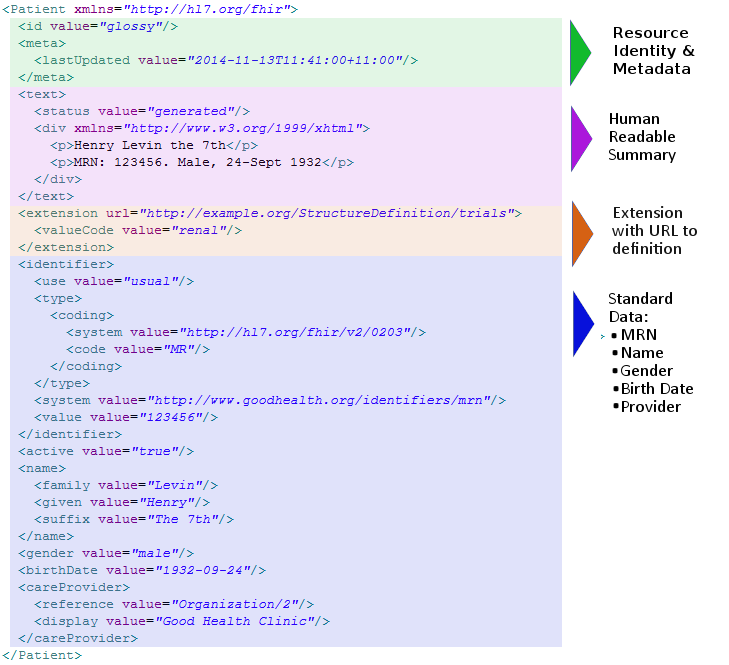
\includegraphics[width=1 \textwidth]{figures/esempio paziente.png}
    \label{fig:esempioPaziente}
    \caption{Esempio risorsa Paziente FHIR}
\end{figure}
\subsubsection{Risorsa Osservazione}
Le osservazioni sono un elemento fondamentale nel mondo sanitario, utili per supportare diagnosi di malattie, monitare progressi
dovuti a cure mediche o determinare pattern ricorrenti nella popolazione.
La maggioranza delle osservazioni possono essere rappresentate da coppie nome-valore coadiuvate da metadati, ma esistono anche tipi di osservazioni con strutture più complesse.
Gli usi della risorsa Osservazione sono molteplici:
\begin{itemize}
    \item Parametri vitali come pressione sanguigna, temperatura corporea o battito cardiaco
    \item Dati di laboratorio derivati da esami medici, come la quantità di glucosio nel sangue
    \item Dati risultanti dallo studio di immagini mediche, come la densità ossea o la misurazione fetale
    \item Sintomatologie cliniche
    \item Misurazioni di macchinari specifici, come elettrocardiogramma o pulsossimetro
    \item Impostazioni di macchinari
    \item Caratteristiche fisiche personali, come ad esempio il colore dei capelli o degli occhi
    \item Storia medica familiare: malattie croniche famigliari, parenti fumatori, etc.
\end{itemize}
Tipicamente, un'osservazione riguarda il soggetto - un paziente, un gruppo di pazienti, una località o un dispositivo - e la distinzione tra il soggetto e ciò che è direttamente
misurato per un'osservazione è specificata nel codice dell'osservazione stessa (ad esempio, "Glucosio nel sangue") e non necessita di essere rappresentata separatamente.
Tuttavia, tre attributi possono essere utilizzati per rappresentare il focus dell'osservazione se non è il soggetto stesso.
\subsubsection*{Profilare un'osservazione}\label{subsubsec:profile}
Nella sua forma più semplice, un'istanza di risorsa può consistere solo di un codice, un valore e un flag di stato.
La rilevanza di altre proprietà varierà in base al tipo di osservazione.
I profili sono creati per fornire linee guida sulla cattura di determinati tipi di osservazioni per un determinato caso d'uso.
La risorsa Osservazione si concentra sul livello di dettaglio catturato dalla maggior parte dei sistemi.
Tuttavia, per un dato caso d'uso, potrebbero esserci vincoli aggiuntivi e informazioni supplementari rilevanti in determinate circostanze.
Come per altre risorse, le estensioni possono essere utilizzate per introdurre questa complessità aggiuntiva.
Il profilo \textbf{FHIR Vital Signs} stabilisce le aspettative minime per la risorsa Osservazione per registrare, cercare e recuperare i segni vitali associati a un paziente, che includono i segni vitali primari oltre a misurazioni aggiuntive come altezza, peso e BMI (Body Mass Index).
Quando un'implementazione FHIR supporta uno qualsiasi dei segni vitali elencati di seguito, l'implementazione dovrà conformarsi a questo profilo per l'osservazione dei parametri vitali.
Un'osservazione che rispetta il profilo appena descritto deve quindi avere:
\begin{itemize}
    \item uno status
    \item un codice appartenente alla categoria "vital signs"
    \item un "valore magico", che descrive cosa l'osservazione sta misurando.
          A tal proposito è necessario specificare che lo standard scelto è \textbf{LOINC} per la sua diffusione capillare
    \item un paziente
    \item una data che indica quando l'osservazione è stata rilevata
    \item un valore numerico e un'unità di misura facente parte dello standard \textbf{UCUM} (Unified Code for Units of Measure)
\end{itemize}
Approfondendo il formato dei valori, è importante specificare che quando un valore di risultato è rappresentato come un concetto predefinito utilizzando un codice, viene utilizzato il datatype valueCodeableConcept.
Questo elemento è vincolato a un set di valori composto da una nomenclatura standard come SNOMED CT o da valori di risultato codificati di un sistema sorgente ("locale").
I risultati possono essere codificati in più set di valori basati su diversi sistemi di codici e questi possono essere mappati utilizzando la risorsa ConceptMap e/o forniti come codifiche aggiuntive direttamente nell'elemento, come mostrato nel listato~\ref{lst:vcc}.
\begin{lstlisting}[caption={Esempio risorsa ConceptMap}, label={lst:vcc}]
            "valueCodeableConcept": {
                "coding": [
                    {
                        "system": "http://snomed.info/sct",
                        "code": "260385009",
                        "display": "Negative"
                    }, {
                        "system": "https://acme.lab/resultcodes",
                        "code": "NEG",
                        "display": "Negative"
                    }
                ],
                "text": "Negative for Chlamydia Trachomatis rRNA"
            }
        \end{lstlisting}
\subsubsection{Esempio osservazione FHIR}
\begin{lstlisting}[caption={Esempio osservazione FHIR}]
    {
        "resourceType": "Observation",
        "id": "body-temperature",
        "meta": {
            "profile": [
                "http://hl7.org/fhir/StructureDefinition/vitalsigns"
            ]
        },
        "text": {
            "status": "generated",
            "div": "<div xmlns=\"http://www.w3.org/1999/xhtml\"><p><b>Generated Narrative: Observation</b><a name=\"body-temperature\">"
        },
        "status": "final",
        "category": [
            {
                "coding": [
                    {
                        "system": "http://terminology.hl7.org/CodeSystem/observation-category",
                        "code": "vital-signs",
                        "display": "Vital Signs",
                        "userSelected": false
                    }
                ],
                "text": "Vital Signs"
            }
        ],
        "code": {
            "coding": [
                {
                    "system": "http://loinc.org",
                    "code": "8310-5",
                    "display": "Body temperature",
                    "userSelected": false
                }
            ],
            "text": "Body temperature"
        },
        "subject": {
            "reference": "Patient/example"
        },
        "encounter": {
            "reference": "Encounter/example"
        },
        "effectiveDateTime": "2024-05-24T10:27:02Z",
        "valueQuantity": {
            "value": 36.5,
            "unit": "C",
            "system": "http://unitsofmeasure.org",
            "code": "Cel"
        }
    }  

\end{lstlisting}
\section{Sviluppo}
Il progetto Java svolto si divide in tre parti: implementazione di classi che modellano osservazioni ACOM,
classe che modella la risorsa osservazione FHIR ed un'interfaccia convertitore, implementata nelle suddette classi ACOM.
Le classi sono state implementate seguendo alcuni concetti fondamentali che distinguono la programmazione ad oggetti:
\begin{itemize}
    \item \textbf{Information hiding} o incapsulamento, tramite la creazione di attributi \textit{private} accedibili tramite metodi get e set.
    \item \textbf{Ereditarietà} implementata seguendo le direttive delle classi descritte dallo standard IEEE 11073-10206 
    \item \textbf{Polimorfismo} tramite la creazione di diversi tipi di costruttori, utili sia durante la creazione di classi derivate sia per nascondere il set di alcuni attributi, gestiti in modo arbitrario per rendere gli oggetti creati più verosimili
\end{itemize}
\subsection{Package ACOM}
\subsubsection{ACOMObservation}\label{subsubsec: ACOMObs}
La classe ACOM Observation fornisce un modello generico per esprimere osservazioni provenienti da dispositivi di salute personali. È basata sul modello di oggetto metrico IEEE 11073-20601 e sui loro attributi concomitanti, nonché sulla risorsa Osservazione di HL7 FHIR. 
Elementi Concettuali di un'osservazione da un Dispositivo di Salute Personale:
\begin{itemize}
    \item Termine di Nomenclatura: identifica cosa rappresenta l'osservazione (ad esempio, temperatura, miglia percorse, energia spesa, pressione sanguigna)
    \item Valore Quantitativo o Codificato dal Sensore: il valore dell'osservazione rilevato dal sensore
    \item Un insieme di modelli per gestire i diversi valori della misurazione
    \begin{itemize}
        \item Scalari: Un numero con un termine di nomenclatura che identifica l'unità dell'osservazione
        \item Discreti: Identifica uno o più valori all'interno di un insieme noto di valori possibili
        \item Campioni Periodici: Una sequenza di quantità scalari periodiche
        \item Stringa: Testo leggibile dall'uomo
        \item Composti: Una misurazione che ha componenti multiple
    \end{itemize}
    \item Timestamp: il tempo della misurazione, generato dall'orologio del PHD. Nel progetto di studio viene utilizzato l'orologio del
        del dispositivo che esegue il codice Java
    \item Informazioni supplementari, se necessarie: Informazioni contestuali aggiuntive che aiutano a perfezionare la comprensione dell'osservazione (ad esempio, media, massimo, minimo, durata, stato, localizzazione corporea, contesto del pasto)
\end{itemize}
Durante lo sviluppo del progetto, è stata sviluppata una classe Java base, \textit{ACOMObservation.java} di tipo astratto poiché funge da genitore per i tipi diversi di misurazioni che le osservazioni possono generare.
Seguendo le direttive dello standard ACOM, si è ritenuto utile per il progetto inserire nella classe \textit{ACOMObservation.java} i seguenti attributi:
\begin{itemize}
    \item \textbf{derivedfrom}
        \begin{itemize}
            \item Nomenclatura: MDC\_ATTR\_OBSERVATION\_REF\_LIST
            \item Descrizione: Indica una relazione tra questa osservazione e una o più altre osservazioni che hanno fornito informazioni formative per questa osservazione 
        \end{itemize}
    \item \textbf{hasmember}
        \begin{itemize}
            \item Nomenclatura: MDC\_ATTR\_EVENT\_CONTEXT
            \item Descrizione: Indica una relazione di raggruppamento tra questa osservazione e una o più altre osservazioni in cui l'osservazione di riferimento è un membro del gruppo di questa osservazione.
            
        \end{itemize}
    \item \textbf{Measurementstatus}
        \begin{itemize}
            \item Nomenclatura:  MDC\_ATTR\_MSMT\_STAT
            \item Descrizione: Indica la validità di un particolare valore o set di campioni.
        \end{itemize}  
    \item \textbf{patient-id}
        \begin{itemize}
            \item Nomenclatura:  MDC\_ATTR\_PERSON\_ID
            \item Descrizione: Un identificatore che permette di associare questa misurazione a una persona. La struttura delle informazioni contenute in questo attributo dipende dal metodo utilizzato per rappresentarle e comunicarle.
        \end{itemize} 
    \item \textbf{Supplementalinformation}
        \begin{itemize}
            \item Nomenclatura:  MDC\_ATTR\_SUPPLEMENTAL\_INFO
            \item Descrizione: Trasmette informazioni supplementari sull'osservazione. Le informazioni supplementari coprono condizioni come la posizione del sensore o la velocità di reazione del soggetto ai cambiamenti. Solo le informazioni che possono essere espresse come termini di nomenclatura possono essere utilizzate in questo attributo.
        \end{itemize} 
    \item \textbf{timestamp}
        \begin{itemize}
            \item Descrizione: Definisce la data e l'ora alla fine del periodo di misurazione. I timestamp devono essere presenti in una misurazione memorizzata. I protocolli di scambio devono definire le semantiche associate al timestamp.
        \end{itemize}
    \item \textbf{type}
        \begin{itemize}
            \item Nomenclatura:  MDC\_ATTR\_ID\_TYPE
            \item Descrizione: Definisce il tipo di misurazione come definito nella nomenclatura (ad esempio, la frequenza del polso per una specifica istanza di oggetto numerico). L'attributo type contiene la partizione della nomenclatura e gli ID del codice termine per un'identificazione estensibile e senza contesto.
        \end{itemize} 
\end{itemize}
Questi attributi permettono una rappresentazione dettagliata e standardizzata delle osservazioni provenienti da dispositivi di salute personali, facilitando l'integrazione e l'interoperabilità dei dati nei sistemi sanitari.
ACOMObservation implementa l'interfaccia \textit{ConverterToFHIR}, parte fondamentale di questo progetto; si è scelto di implementare quest'interfaccia nella classe base per poi andare ad effettuare l'override nelle classi che modellano le specializzazioni approfondite.
Vengono introdotte ora le classi che estendono ACOMObservation presenti nel progetto.
\begin{figure}[H]
    \centering
    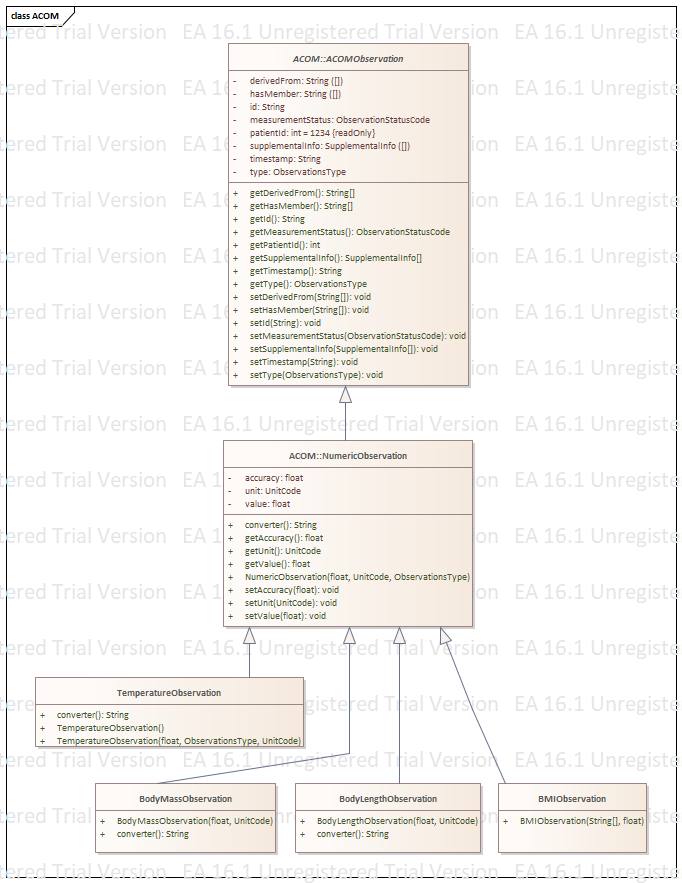
\includegraphics[width=12cm, height=20cm]{figures/ACOM.png}
    \caption{Classi presenti nel package ACOM}
    \label{fig:Acom}
\end{figure}
\subsubsection{NumericObservation}
La classe NumericObservation modella un'osservazione numerica, ad esempio un'osservazione di temperatura o di peso. 
\begin{figure}[H]
    \centering
    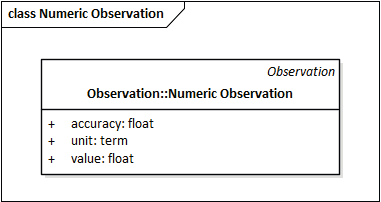
\includegraphics[width=1\linewidth]{figures/image.png}
    \caption{Classe Numeric Observation}
    \label{fig:numeric-observation}
\end{figure}
Gli attributi con cui estende ACOMObservation sono:
\begin{itemize}
    \item value, contiene il valore numerico dell'osservazione
    \item unit, descrive l'unità di misura dell'osservazione tramite l'utilizzo della nomenclatura descritta nel paragrafo~\ref{subsec:PackageUtil}.
    \item accuracy, descrive il livello di accuratezza dell'osservazione in percentuale
\end{itemize}
\'E presente anche un costruttore, con parametri value, unit e type, utile nelle estensioni della classe che modellano le specializzazioni.
Si tratta di una delle classi più rilevanti dell'intero progetto, poiché sarà la base per lo sviluppo delle specializzazioni sviluppate, le osservazioni dei dispositivi termometro e Bilancia con altimetro, presentati in seguito.
\subsubsection{Classi specializzazioni}
\subsubsection*{TemperatureObservation}
Classe che modella l'osservazione della temperatura corporea compiuta da un termometro in diverse parti del corpo, come bocca, ascella, dito, etc.
Estende la classe NumericObservation, senza però aggiungere attributi, poiché possiede la stessa struttura. Sviluppa dunque due costruttori, uno senza parametri utile per i primi test e simulazioni ed uno che accetta i tre parametri fondamentali di NumericObservation: value, unit e type; entrambi utilizzano il costruttore della classe padre per settare gli attributi ereditati.
Si è scelto di gestire in modo automatico la creazione altri parametri, come timestamp, per emulare lo scambio di informazioni che avviene tra il sistema che gestisce l'orologio ed il generatore di osservazioni di un vero PHD.
TemperatureObservation effettua l'override dell'interfaccia \textit{ConverterToFHIR}, ereditata dalla classe antenata ACOMObservation; la sua implementazione verrà presentata nel dettaglio nel paragrafo~\ref{subsubsec:ConverterToFHIR}.
Viene fornito ora nel listato~\ref{lst:to} un esempio di un'istanza della classe TemperatureObservation.
\begin{lstlisting}[caption={Esempio istanza di TemperatureObservation},label={lst:to}]
    {
        "accuracy": 0.1,
        "value": 36.5,
        "unit": "MDC_DIM_DEGC",
        "id": "9d9835d6-da4b-4d37-aa94-ba40f260ec10",
        "patientId": 1234,
        "timestamp": "2024-05-24T10:27:02Z",
        "type": "MDC_TEMP_BODY"
    }
\end{lstlisting}
\subsubsection*{BodyMassObservation}
Classe che modella l'osservazione della massa corporea.
Estende la classe NumericObservation, senza però aggiungere attributi, poiché possiede la stessa struttura.
Sviluppa un costruttore che accetta i tre parametri fondamentali di NumericObservation: value, unit e type; utilizza il costruttore della classe padre per settare gli attributi ereditati.
Si è scelto di gestire in modo automatico la creazione altri parametri, come timestamp, per emulare lo scambio di informazioni che avviene tra il sistema che gestisce l'orologio ed il generatore di osservazioni di un vero PHD.
BodyMassObservation effettua l'override dell'interfaccia \textit{ConverterToFHIR}, ereditata dalla classe antenata ACOMObservation; la sua implementazione verrà presentata nel dettaglio nel paragrafo~\ref{subsubsec:ConverterToFHIR}.
Viene fornito ora nel listato~\ref{lst:bmo} un esempio di un'istanza della classe BodyMassObservation.
\begin{lstlisting}[caption={Esempio istanza di BodyMassObservation},label={lst:bmo}]
    {
        "accuracy": 0.1,
        "value": 66.0,
        "unit": "MDC_DIM_KILO_G",
        "id": "dad403fa-7716-44db-bcc7-35aea995d39a",
        "patientId": 1234,
        "timestamp": "2024-06-11T12:19:54Z",
        "type": "MDC_MASS_BODY_ACTUAL"
    }
\end{lstlisting}
\subsubsection*{BodyLengthObservation}
Classe che modella l'osservazione dell'altezza corporea.
Estende la classe NumericObservation, senza però aggiungere attributi, poiché possiede la stessa struttura.
Sviluppa un costruttore che accetta i tre parametri fondamentali di NumericObservation: value, unit e type; utilizza il costruttore della classe padre per settare gli attributi ereditati.
Si è scelto di gestire in modo automatico la creazione altri parametri, come timestamp, per emulare lo scambio di informazioni che avviene tra il sistema che gestisce l'orologio ed il generatore di osservazioni di un vero PHD.
BodyLengthObservation effettua l'override dell'interfaccia \textit{ConverterToFHIR}, ereditata dalla classe antenata ACOMObservation; la sua implementazione verrà presentata nel dettaglio nel paragrafo~\ref{subsubsec:ConverterToFHIR}.
Viene fornito ora nel listato~\ref{lst:blo} un esempio di un'istanza della classe BodyLengthObservation.
\begin{lstlisting}[caption={Esempio istanza di BodyLengthObservation},label={lst:blo}]
    {
        "accuracy": 0.1,
        "value": 66.0,
        "unit": "MDC_DIM_KILO_G",
        "id": "dad403fa-7716-44db-bcc7-35aea995d39a",
        "patientId": 1234,
        "timestamp": "2024-06-11T12:19:54Z",
        "type": "MDC_MASS_BODY_ACTUAL"
    }
\end{lstlisting}
\subsubsection*{BMIObservation}
Classe che modella l'osservazione del rapporto tra altezza e massa corporea.
Necessita dunque della presenza di due osservazioni, una per la massa ed una per l'altezza, che verranno collegate alla BMI tramite il suo attributo \textit{derived-from}.
Estende la classe NumericObservation, senza però aggiungere attributi, poiché possiede la stessa struttura.
Sviluppa un costruttore che accetta i tre parametri fondamentali di NumericObservation: value, unit e type; utilizza il costruttore della classe padre per settare gli attributi ereditati.
Si è scelto di gestire in modo automatico la creazione altri parametri, come timestamp, per emulare lo scambio di informazioni che avviene tra il sistema che gestisce l'orologio ed il generatore di osservazioni di un vero PHD.
BodyLengthObservation effettua l'override dell'interfaccia \textit{ConverterToFHIR}, ereditata dalla classe antenata ACOMObservation; la sua implementazione verrà presentata nel dettaglio nel paragrafo~\ref{subsubsec:ConverterToFHIR}.
Viene fornito ora nel listato~\ref{lst:bmio} un esempio di un'istanza della classe BMIObservation.
\begin{lstlisting}[caption={Esempio istanza di BMIObservation},label={lst:bmio}]
    {
        "accuracy": 0.1,
        "value": 35.0,
        "unit": "MDC_DIM_KILO_G_PER_M_SQ",
        "id": "5e17639c-893c-4766-9afd-7275aa6e6f05",
        "derivedFrom": [
            "1ee1fb5c-80c3-4be6-af2c-c773638a5663",
            "a2f8d3fc-416c-4f2c-a75a-885e47e34531"
        ],
        "patientId": 1234,
        "timestamp": "2024-07-12T18:21:34Z",
        "type": "MDC_RATIO_MASS_BODY_LEN_SQ"
    }
\end{lstlisting}
\subsection{Package FHIR}
\subsubsection{FHIRObservation}
La classe FHIRObservation è stata implementata seguendo le specifiche contenute nella guida d'implementazione di FHIR \cite{FHIROBSERVATION}.
A differenza dello standard IEEE 11073-10206 ACOM, creato allo scopo di modellare un sistema astratto, FHIR basa la sua filosofia implementativa sul concetto di risorsa, come già illustrato nel paragrafo~\ref{subsec: FHIR}.
Si è resa necessaria quindi la creazione di diversi datatypes, utili a descrivere le risorse che compongono un'osservazione FHIR, tramite lo sviluppo di classi Java, presentate nei successivi paragrafi.
La classe FHIRObservation contiene dunque i seguenti attributi:
\begin{itemize}
    \item \textbf{resourceType}, stringa che descrive il tipo di risorsa;
    \item \textbf{id}, stringa che contiene un codice identificativo della risorsa.
    \item \textbf{meta}, datatype modellato dalla classe Meta. Composto da un ArrayList di stringhe chiamato profile, contiene il riferimento URL al profilo (concetto descritto nel paragrafo~\ref{subsubsec:profile}) \textit{vitalsigns} che permette ai sistemi IT di verificare la struttura dell'osservazione in esame
    \item \textbf{text}, datatype modellato dalla classe Text. Composto da due stringhe: status e div.
    contiene la parte humam readable dell'osservazione, cioè la descrizione a parole del contenuto dell'osservazione.
    \item \textbf{status}, stringa che contiene lo stato dell'osservazione
    \item \textbf{code}, datatype modellato dalla classe CodeableConcept. Composto da un arrayList del datatype Coding, modellato dalla classe Coding, e da text, una stringa.
    Coding è composto da quattro stringhe:
    \begin{itemize}
        \item \textbf{system}, contiene il tipo di sistema di cui il codice fa parte
        \item \textbf{version}, contiene la versione del sistema
        \item \textbf{code}, contiene il valore del codice 
        \item \textbf{display}, contiene la versione human readable del codice
    \end{itemize}
    Il datatype Coding contiene le informazioni necessarie per descrivere la categoria dell'osservazione.
    Di conseguenza code contiene uno o più elementi Coding, poiché lo standard FHIR supporta molteplici standard di codici sanitari.
    \item \textbf{category}, comporto da arrayList di datatype CodeableConcept, lo stesso dell'attributo code. La differenza tra gli attributi code e category sta nella funzione che ricoprono: category si occupa di descrivere la categoria di osservazione, mentre code si occupa di descrivere il tipo di osservazione in uno o più standard medici.
    \'E importante sottolineare come il tipo sia un sottoinsieme della categoria.
    \item \textbf{subject}, datatype modellato dalla classe Person. Composto da una stringa, reference, che contiene il riferimento al tipo di persona citata, nel caso specifico il paziente da cui è stata presa l'osservazione.
    \item \textbf{encounter}, datatype modellato dalla classe Person. Composto da una stringa, reference, che contiene il riferimento al tipo di persona citata, nel caso specifico l'operatore sanitaro che ha effettuato l'osservazione.
    \item \textbf{effectiveDateTime}, stringa che contiene la data in cui è stata generata l'osservazione.
    \item \textbf{valueQuantity}, datatype modellato dalla classe Quantity. Composto da un attributo value di tipo float e quattro stringhe:
    \begin{itemize}
        \item comparator, opzionale, contiene uno dei simboli utili per interpretare il valore numerico: <,<=,=>,> 
        \item unit, contiene l'unità di misura del valore numerico
        \item system, contiene il sistema di riferimento da cui è presa l'unità di misura
        \item code, contiene il codice dell'unità di misura del valore numerico
    \end{itemize}
    valueQuantity è un degli attributi fondamentali dell'osservazione, in quanto contiene le informazioni sull'effettivo valore della rilevazione.
    \item \textbf{dataAbsentReason}, modellato dall'enumerazione ObservationStatusCode, descritta nel paragrafo~\ref{subsec:PackageUtil}.
    Questo attributo è presente solo nel caso in cui non sia presente l'attributo valueQuantity, specifica il motivo per cui il valore manca
    Altri attributi che sono stati modellati, ma che non vengono utilizzati dal progetto:
    \begin{itemize}
        \item \textbf{interpretation}, modellato dall'enumerazione ObservationStatusCode, presentata nel paragrafo~\ref{subsec:PackageUtil}. Contiene il codice che descrive l'interpretazione da dare al valore dell'osservazione
        \item \textbf{derivedFrom} arrayList di stringhe, contiene le possibili osservazioni
        da cui l'osservazione in esame è derivata
        \item \textbf{hasMember} arrayList di stringhe, contiene le possibili osservazioni che fanno parte dell'osservazione in esame
        \item \textbf{component}, modellato dall'enumerazione SupplementalInfo, presentata nel paragrafo~\ref{subsec:PackageUtil}. Contiene i codici di eventuali componenti aggiuntive dell'osservazione in esame
    \end{itemize}
\end{itemize}
\begin{figure}[H]
    \centering
    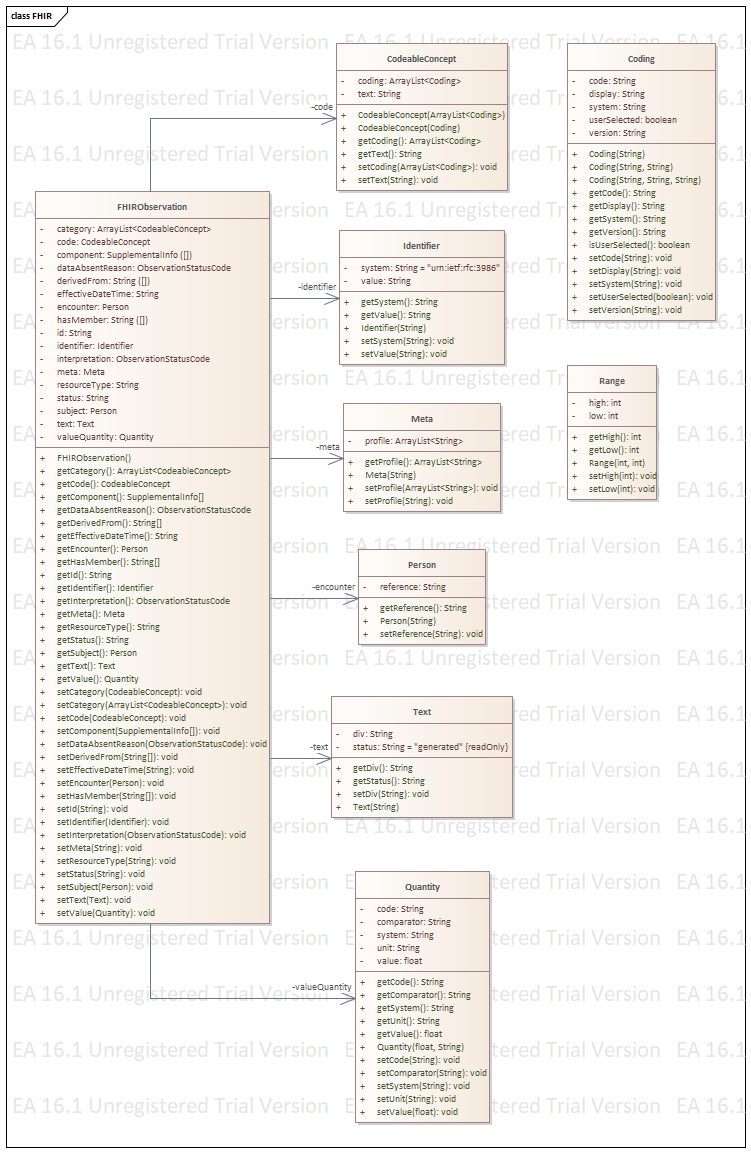
\includegraphics[width=1\linewidth]{figures/FHIR.png}
    \caption{Classi presenti nel package FHIR}
    \label{fig:fhir}
\end{figure}
\subsection{Interfaccia ConverterToFHIR}\label{subsubsec:ConverterToFHIR}
L'interfaccia ConverterToFHIR sfrutta la struttura delle osservazioni che il formato di partenza IEEE 11073-10206 ACOM produce, poiché sono state implementate appositamente per permettere il mapping degli attributi con il formato d'arrivo FHIR.
Si è scelto dunque di creare una semplice interfaccia, ConverterToFHIR, formata da un unico metodo (ma idealmente espansibile con altri) chiamato converter e di implementarlo nella classe base ACOMObservation, presentata nel paragrafo~\ref{subsubsec: ACOMObs}; di conseguenza tutte le classi derivate avranno la loro interfaccia, permettendo di sviluppare converter dedicati per ogni specifica.
Poiché la struttura logica del convertitore è simile, verrà presentata una sola volta per poi mostrare nei prossimi paragrafi le tre differenti implementazioni.
Il metodo converter è di tipo string, poiché restituirà l'istanza della classe FHIRObservation codificata in formato JSON utilizzando la libreria Gson~\cite{GSON}; questa scelta permette il salvataggio delle osservazioni tradotte in un file JSON, come presentato nel paragrafo~\ref{subsec:Main}.
Tramite il costruttore della classe FHIRObservation vengono settati alcuni attributi che hanno un valore standard.
Gli attributi vengono poi divisi in due categorie essenziali: attributi che dipendono dal tipo di osservazione,id, meta, text, category e code, ed attributi che dipendono dal valore dell'osservazione, effectiveDateTime, valueQuantity.
Come è possibile riscontrare dal codice presente nei prossimi paragrafi, vengono prima mappati gli attributi che appartengono alla prima categoria, in seguito gli attributi che appartengono alla seconda.
\subsubsection*{Implementazione nella classe TemperatureObservation}
\begin{lstlisting}[language= Java, caption = Metodo converter per la classe TemperatureObservation]
    // https://hl7.org/fhir/observation-example-body-temperature.json.html
    @Override
    public String converter() {
        FHIRObservation fhirObservation = new FHIRObservation();
        // parametri che non dipendono da valori presenti nell'osservazione ACOM, ma che possiamo settare in base al tipo di osservazione
        fhirObservation.setId("body-temperature");
        fhirObservation.setMeta("http://hl7.org/fhir/StructureDefinition/vitalsigns");
        fhirObservation.getText().setDiv(
                "<div xmlns=\"http://www.w3.org/1999/xhtml\"><p><b>Generated Narrative: Observation</b><a name=\"body-temperature\">");
        Coding[] coding = new Coding[2];
        // category
        coding[0] = new Coding("http://terminology.hl7.org/CodeSystem/observation-category",
                Costants.CODE_VITAL_SIGNS, Costants.DISPLAY_VITAL_SIGNS);
        CodeableConcept category = new CodeableConcept(coding[0]);
        category.setText(Costants.DISPLAY_VITAL_SIGNS);
        fhirObservation.setCategory(category);

        // code
        coding[1] = new Coding("http://loinc.org", "8310-5", "Body temperature");
        CodeableConcept code = new CodeableConcept(coding[1]);
        code.setText("Body temperature");
        fhirObservation.setCode(code);
        // effectiveDateTime
        fhirObservation.setEffectiveDateTime(this.getTimestamp());
        // value
        Quantity valueQuantity = new Quantity(this.getValue(), "http://unitsofmeasure.org");
        switch (this.getUnit()) {
            case MDC_DIM_DEGC: {
                valueQuantity.setUnit("C");
                valueQuantity.setCode(Costants.CODE_TEMP_CEL);
                break;
            }
            case MDC_DIM_FAHR:
                valueQuantity.setUnit("F");
                valueQuantity.setCode(Costants.CODE_TEMP_FAHR);
                break;
            case MDC_DIM_KELVIN:
                valueQuantity.setUnit("K");
                valueQuantity.setCode(Costants.CODE_TEMP_KEL);
                break;
            default:
                break;
        }
        fhirObservation.setValue(valueQuantity);
        Gson gson = new GsonBuilder().disableHtmlEscaping().create();
        String json = gson.toJson(fhirObservation);
        return json;
    }
\end{lstlisting}
\subsubsection*{Implementazione nella classe BodyMassObservation}
\begin{lstlisting}[language = Java, caption = metodo converter per la classe BodyMassObservation]
    @Override
    public String converter() {
        FHIRObservation fhirObservation = new FHIRObservation();
                // parametri che non dipendono da valori presenti nell'osservazione ACOM, ma che
        // possiamo settare in base al tipo di osservazione
        fhirObservation.setId("body-weight");
        fhirObservation.setMeta("http://hl7.org/fhir/StructureDefinition/vitalsigns");
        fhirObservation.getText().setDiv(
                "<div xmlns=\"http://www.w3.org/1999/xhtml\"><p><b>Generated Narrative: Observation</b><a name=\"body-weight\">");
        
        // category
        CodeableConcept category = new CodeableConcept(new Coding("http://terminology.hl7.org/CodeSystem/observation-category",
        Costants.CODE_VITAL_SIGNS, Costants.DISPLAY_VITAL_SIGNS));
        category.setText(Costants.DISPLAY_VITAL_SIGNS);
        fhirObservation.setCategory(category);

        // code
        ArrayList<Coding> coding = new ArrayList<>();
        coding.add(new Coding("http://loinc.org", "29463-7", "Body Weight"));
        coding.add(new Coding("http://loinc.org","3141-9", "Body weight Measured"));
        coding.add(new Coding("http://snomed.info/sct","27113001","Body weight"));
        coding.add(new Coding("http://acme.org/devices/clinical-codes","body-weight","Body Weight"));
        CodeableConcept code = new CodeableConcept(coding);
        fhirObservation.setCode(code);
        
        // effectiveDateTime
        fhirObservation.setEffectiveDateTime(this.getTimestamp());

        // value
        Quantity valueQuantity = new Quantity(this.getValue(), "http://unitsofmeasure.org");
        switch (this.getUnit()) {
            case MDC_DIM_KILO_G: {
                valueQuantity.setUnit("kg");
                valueQuantity.setCode(Costants.CODE_WEIGHT_KILO_G);
                break;
            }
            case MDC_DIM_LB:
                valueQuantity.setUnit("lbs");
                valueQuantity.setCode(Costants.CODE_WEIGHT_LBS);
                break;
            default:
                break;
        }
        fhirObservation.setValue(valueQuantity);
        Gson gson = new GsonBuilder().disableHtmlEscaping().create();
        String json = gson.toJson(fhirObservation);
        return json;
    }

\end{lstlisting}
\subsubsection*{Implementazione nella classe BodyLengthObservation}
\begin{lstlisting} [language = Java, caption = metodo converter per la classe BodyLengthObservation]
    @Override
    public String converter() {
        FHIRObservation fhirObservation = new FHIRObservation();
                // parametri che non dipendono da valori presenti nell'osservazione ACOM, ma che
        // possiamo settare in base al tipo di osservazione
        fhirObservation.setId("body-length");
        fhirObservation.setMeta("http://hl7.org/fhir/StructureDefinition/vitalsigns");
        fhirObservation.getText().setDiv(
                "<div xmlns=\"http://www.w3.org/1999/xhtml\"><p><b>Generated Narrative: Observation</b><a name=\"body-length\">");
        
        // category
        CodeableConcept category = new CodeableConcept(new Coding("http://terminology.hl7.org/CodeSystem/observation-category",
        Costants.CODE_VITAL_SIGNS, Costants.DISPLAY_VITAL_SIGNS));
        category.setText(Costants.DISPLAY_VITAL_SIGNS);
        fhirObservation.setCategory(category);

        // code
        ArrayList<Coding> coding = new ArrayList<>();
        coding.add(new Coding("http://loinc.org", "8302-2", "Body height"));
        coding.add(new Coding("http://loinc.org","8306-3", "Body height --lying"));
       
        CodeableConcept code = new CodeableConcept(coding);
        fhirObservation.setCode(code);
        fhirObservation.getCode().setText("Body Length");
        
        // effectiveDateTime
        fhirObservation.setEffectiveDateTime(this.getTimestamp());

        // value
        Quantity valueQuantity = new Quantity(this.getValue(), "http://unitsofmeasure.org");
        switch (this.getUnit()) {
            case MDC_DIM_CENTI_M: {
                valueQuantity.setUnit("cm");
                valueQuantity.setCode(Costants.CODE_WEIGHT_CENTI_M);
                break;
            }
            case MDC_DIM_INCH:
                valueQuantity.setUnit("inch");
                valueQuantity.setCode(Costants.CODE_WEIGHT_INCH);
                break;
            default:
                break;
        }
        fhirObservation.setValue(valueQuantity);
        Gson gson = new GsonBuilder().disableHtmlEscaping().create();
        String json = gson.toJson(fhirObservation);
        return json;
    }
\end{lstlisting}
\subsection{Package Util}\label{subsec:PackageUtil}
\subsubsection*{Gestione della nomenclatura}
Durante lo sviluppo del progetto si è ritenuto utile creare alcune enumerazioni, allo scopo di gestire separatamente i diversi ambiti della nomenclatura:
\begin{itemize}
    \item ObservationStatusCode, codici per determinare lo status della macchina che ha prodotto l'osservazione
    \item ObservationType, codici per determinare il tipo di osservazione
    \item SupplementalInfo, codici per determinare la presenza di informazioni aggiuntive all'interno dell'osservazione
    \item UnitCode, codici per determinare l'unità di misura del valore osservato
\end{itemize}
\'E presente anche una classe "container", Costants, che come suggerisce il nome contiene alcune stringhe utili in alcuni contesti. 
\subsection{Classe Main}\label{subsec:Main}
La classe Main svolge un importante compito: simula, semplificandolo, il sistema formato da PHD e il PHG (solitamente un cellulare, tramite un applicazione) e il conseguente scambio di informazioni.
Tramite la lettura di un file JSON, in cui sono salvate le osservazioni in formato ACOM, viene simulata la ricezione di dati provenienti da PHD da parte del PHG.
\'E divisa in tre sezioni principali:
\begin{itemize}
    \item lettura da file JSON di osservazioni ACOM
    \item creazione di nuove osservazioni ACOM
    \item conversione in formato FHIR delle osservazioni lette e salvataggio nei file JSON, uno dedicato al formato ACOM ed uno dedicato al formato FHIR
\end{itemize}
Le osservazioni, lette tramite l'utilizzo della libreria JsonReader~\cite{JsonReader}, vengono salvate in arrayList di tipo ACOMObservation, che accetta dunque qualsiasi tipo di osservazione.
Viene poi proposto un menu, che permette di scegliere la specifica di osservazione ACOM da generare e successivamente i valori che essa conterrà.
Infine, nel caso in cui siano effettivamente state create nuove osservazioni, vengono convertite in formato FHIR, sovrascrivendo in seguito il file di input con osservazioni ACOM e il file di output contenente le osservazioni FHIR.
Tale file può rappresentare l'elaborazione che il PHG effettua sui dati, prima di inviarli ad un cloud che accetta dati in formato FHIR.
\subsection{Validazione osservazioni FHIR}
Al termine dello sviluppo del progetto di tesi, si è proceduto a verificare, tramite il validatore ufficiale fornito dall'associazione HL7~\cite{FHIRVALIDATOR}, delle osservazioni prodotte, ottenendo la conferma della correttezza dei dati.
\\
\section{Conclusione}
Questo progetto di tesi presenta una prima versione dello sviluppo di un convertitore universale da ACOM a FHIR, implementato su due particolari specifiche della famiglia di standard IEEE 11073: IEEE 11073-10208 e IEEE 11073-10415.
Tuttavia, esistono molti altre osservazioni generate da dispositivi medici.
Sarebbe quindi utile approfondire il progetto modellando come specificato dallo standard ACOM anche i dispositivi medici con le relative osservazioni, così da ottenere una simulazione realistica del sistema reale, introducendo successivamente anche una vera comunicazione tramite Bluetooth.

\newpage
\printbibliography

\newpage
\section*{Ringraziamenti}
Al termine di questo lavoro, desidero ringraziare la professoressa Daniela Micucci per l’opportunità di
ricerca presso il DISCo (Dipartimento di Informatica, Sistemistica e Comunicazione) e il dott. Giovanni Donato Gallo per avermi seguito costantemente durante le fasi di stage e di stesura della tesi.
Successivamente, ci tengo a ringraziare chi è stato al mio fianco durante questo percorso universitario: in primis la mia famiglia, per il sostegno dato durante il percorso universitario; i miei amici e compagni di viaggio Nicola e Radu, con cui ho condiviso i traguardi e le fatiche in questi anni; tutti i compagni universitari con cui ho lavorato a compiti e progetti.
Infine ringrazio Silvia, per avermi accompagnato in questo percorso con il suo affetto ed i tanti consigli preziosi.

\end{document}